  {\color{teal!90}\chapter{AirPlay Server}\label{cap:AirPlayServer}}

  \AddToShipoutPictureBG*{%
    \AtPageUpperLeft{%
      \raisebox{-\height}{%
        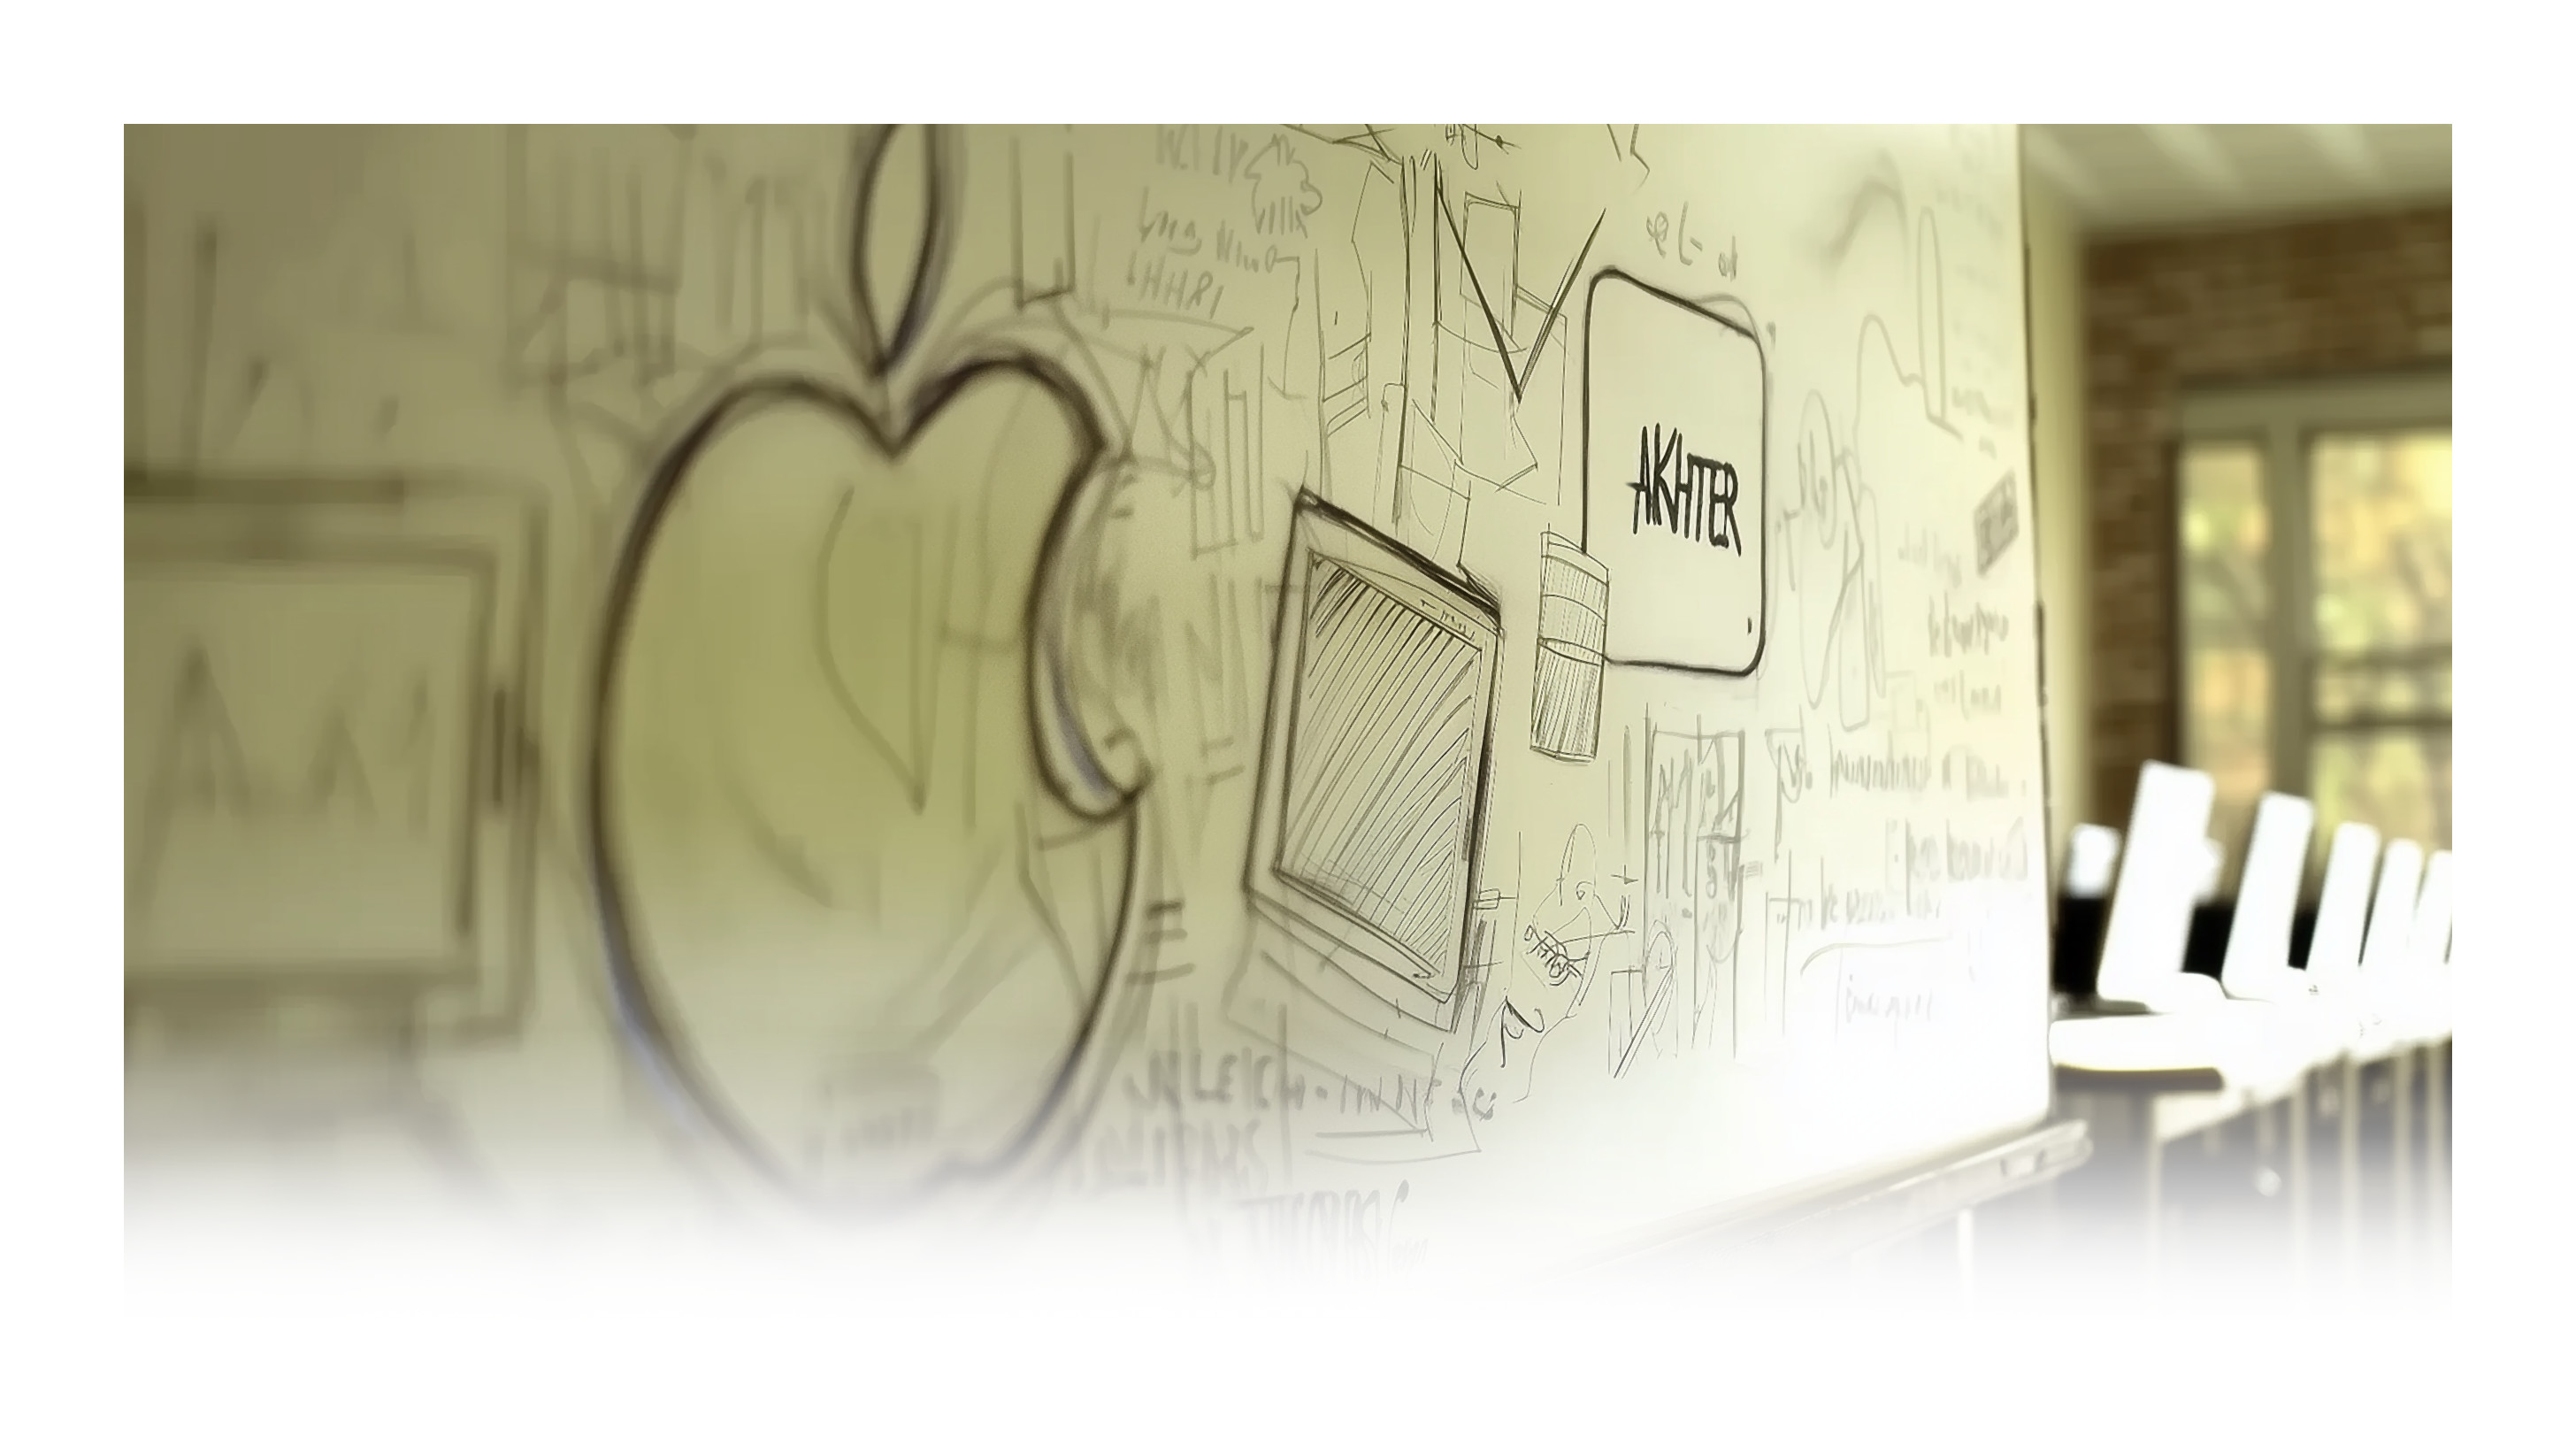
\includegraphics[width=\paperwidth]{./chapters/classroom.jpg}%
      }%
    }
  }

  \minitoc % Creating an actual mini table of contents

  \section{Overview of the AirPlay Server}
  \label{sec:OverviewAirPlayServer}

  This chapter delves into the implementation of the \texttt{AirPlayServer}, a foundational class responsible for facilitating AirPlay interactions. Below is a diagram showing its structure:

  \begin{center}
    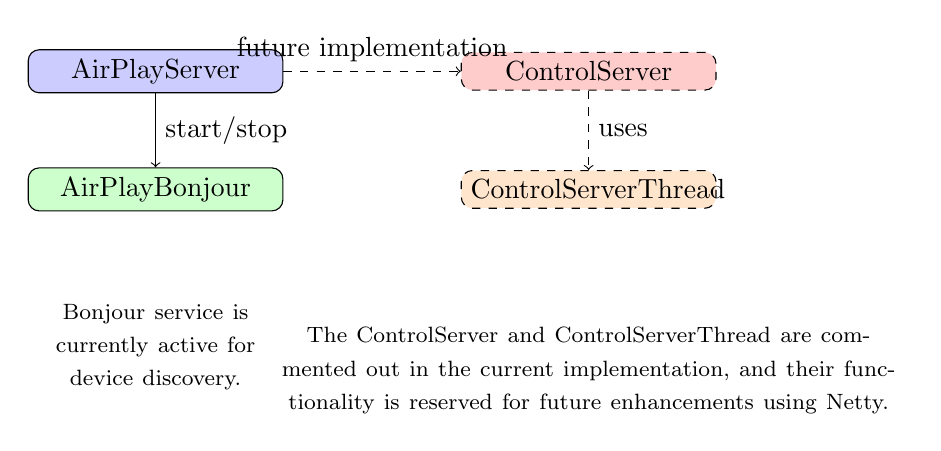
\begin{tikzpicture}[node distance=1.5cm, auto]
      % Nodes
      \node[draw, rounded corners, text centered, text width=3cm, fill=blue!20] (airplayserver) {AirPlayServer};
      \node[draw, rounded corners, text centered, text width=3cm, below of=airplayserver, fill=green!20] (bonjour) {AirPlayBonjour};
      \node[draw, dashed, rounded corners, text centered, text width=3cm, right of=airplayserver, xshift=4cm, fill=red!20] (controlserver) {ControlServer};
      \node[draw, dashed, rounded corners, text centered, text width=3cm, below of=controlserver, fill=orange!20] (controlthread) {ControlServerThread};

      % Connections
      \draw[->] (airplayserver) -- node[midway, right] {start/stop} (bonjour);
      \draw[->, dashed] (airplayserver) -- node[midway, above] {future implementation} (controlserver);
      \draw[->, dashed] (controlserver) -- node[midway, right] {uses} (controlthread);

      % Annotations
      \node[below of=bonjour, yshift=-0.5cm, text width=3cm, align=center] (note1)
      {\footnotesize Bonjour service is currently active for device discovery.};

      \node[below of=controlthread, yshift=-0.8cm, text width=8cm, align=center] (note2)
      {\footnotesize The ControlServer and ControlServerThread are commented out in the current implementation, and their functionality is reserved for future enhancements using Netty.};
    \end{tikzpicture}
  \end{center}

  The diagram illustrates how the \texttt{AirPlayServer} initializes and manages the Bonjour service while leaving space for a future \texttt{ControlServer} integration. The current implementation focuses on network discovery using Bonjour, with plans to handle media streaming in subsequent iterations.

  \section{Initialization and Parameters}
  \label{sec:InitializationParameters}

  The \texttt{AirPlayServer} is constructed with the following parameters:
  \begin{itemize}
    \item \texttt{serverName}: The name of the server, used for network identification.
    \item \texttt{airPlayPort}: The port for AirPlay communications, defaulting to \texttt{7000}.
    \item \texttt{airTunesPort}: The port for AirTunes communications, defaulting to \texttt{49152}.
    \item \texttt{airplayDataConsumer}: An interface for handling incoming media data.
  \end{itemize}
